\chapter{Experiment}
Although many algorithms have been proposed to tackle the meta-search merging problem, not all of them have been tested in real world environments. Some information or statistics that needed by an algorithm is not available in some situations. So the feasibilities of these algorithms remain unknown. On the other hand, many algorithms proposed with an ambition to promote the performance of the system on TREC test collection. So even if an algorithm can outperform other algorithms within TREC among any topic, it is not sufficient to say the algorithm is good enough to solve the problem. In this section, we develop an evaluation platform based on a real world system to test the feasibility of different algorithms as well as the performance of these algorithms.

\section{Test Collection and Queries}
Many of previous works in meta-search were tested based on some standard test collections like TREC and GOV2. Typically, these test collections are composed by \textit{document collections}, \textit{information needs} expressed by the queries as well as the \textit{relevance score} of the queries and documents. And the evaluation procedures judge the ranking results following a particular algorithm compared to relevance score. However, the test collection approach is very different from a real world situation in some sense. First of all, the documents exist in the collections are static and do not change over time, which is quite different from the situation when we search documents in a web search engine. And documents format in real world varies, and information provided by different search engines are different from each other. For example, when search information of a person, the ANU contact web returns a list of contacts with names and contact numbers while the ANU website returns the title of related documents as well as a summary of the documents.So the retrieved information is quite biased. The other information provided by the test collection is the relevance score assessed by the experts. TREC comes with a set of natural language statements of information needs, named topics\cite{Voorhees1999}. These topics that carefully defined by an assessor who would also evaluate the relevance of the topic and documents. Topics are expressed by query terms that are carefully constructed to make sure that it is clear. However, the information needs may be ambiguous in a real world situation due to the fact users may not be able to express their needs in accurate queries, which may bring inaccuracy results to the relevance judgement\cite{Thomas2006}. And what is more significant issue is that many of previous merging algorithms have not been tested in a real world environment. Some of the algorithms will perform variously in a different situation or even cannot work in such a situation. So in this paper, we built a platform based on a real world environment.

\subsection{Experiment Environment}
To construct a real world environment for evaluating different merging algorithms, we built an evaluation test bed based on the websites of the Australian National University. There exists many sites of different departments of the Australian National University. However, some websites are totally distributed from others and there exists no access point to the resources from other sites. And the university do not provide an integrated interface for users to get access to all the resources. 
\subsubsection{Document Source}
We picked 7 sites that are distributed from each other, each of which has their own documents repository and has a search interface for users to access the resources.

\begin{table}
\begin{tabular}{|p{3cm}|p{5cm}|p{8cm}|}
\hline 
Collection & Description & Location \\ 
\hline 
ANU Search & The main entry of the university, containing information of people, news as well as some information in research & http://search.anu.edu.au/ \\ 
\hline 
ANU Contact Search & The site contains information of contacts as well as positions of a stuff   & http://www.anu.edu.au/dirs\\ 
\hline 
ANU Map & The site provides information of locations on campus & http://campusmap.anu.edu.au/ \\ 
\hline 
ANU Library & The library catalogue of ANU & http://anulib.anu.edu.au/ \\ 
\hline 
ANU Study & Course information of ANU & https://studyat.anu.edu.au \\ 
\hline 
ANU Research & The site provide researcher, research project and research publication information of ANU, the three types of resources are actually separated into different collections, so it has been built into three different collections & https://researchers.anu.edu.au/ \\ 
\hline 
ANU Dspace & Document information related to ANU & https://digitalcollections.anu.edu.au/ \\ 
\hline 
\end{tabular} 
\caption{Internal Collections}
\label{table:internal collection}
\end{table}

Apart from these collections existing inside the university, we also import other two collection which can regard as a special case of meta-search. We add two social media site that is related to ANU as shown in Table \ref{table:External collection}.These two social media site, on the other hand, gave us an opportunity to examine the performance of different merging algorithms in on a real time environment. Also, the contents in these site are not text only, many other formats of information exist in both internal and external collections. However, we claim that all the algorithms that we applied is based on the text information.

\begin{table}
\begin{tabular}{|p{3cm}|p{5cm}|p{8cm}|}
\hline 
Collection & Description & Location \\ 
\hline 
ANU Youtube Channel & The official Youtube Channel of ANU & http://www.youtube.com/user/ANUchannel \\ 
\hline 
ANU Twitter Channel  &The official Twitter Channel of ANU & https://twitter.com/ANUmedia\\ 
\hline
\end{tabular} 
\caption{External Collections}
\label{table:External collection}
\end{table}
\subsubsection{Document Overlap}
Although the document collections are distributed from each other, there still exists some documents overlap between these document repositories. For example, there exists limited amount of documents overlap between ANU website and ANU study at website. Also, the results in ANU website collection may contain some documents retrieved form ANU research. And some other types of document overlap also exists, documents are accessible to many collections but formatted differently. For example, the ANU website may contain videos from youtube site together with some text description. However, the amount of document overlap is very limited and we ignored the little overlap in our experiments.

\subsection{Building test collection} 
Previous evaluation of new algorithms are mostly based on a large standard test collection. However, in our case, no test collection is provided. Although there exist some methods that can compare performance of different information retrieval system without a test collection \cite{Thomas2006}. However, these methods are basic based on the judgement that a user given to say if a system is better than the other, which may not provide sufficient evidence to convince. And as the collections changes over time, we cannot ask assessors to judge documents at a time and conduct the evaluation experiment at the other time. And as the judgement procedure can really take a lot of time, many issues can arise during the procedure, some documents may be deleted while some other pages can be created during the time, especially in the case of social media system. 

So the solution is creating a test collection ourselves. There exist large volumes of documents in each collections, so it would be a large collection of documents if we run a full document collection. And also, due the limitation of bandwidth and disk space, it is not feasible to put all documents into the test collection. And on the other hand, the document judgement procedure will take too much time. Later in the experiment, what we care is the ranking of documents that is already retrieved by each collection when search a particular query or topic. So the necessary and useful documents are those document retrieved by the meta-search system on those queries defined in advance. Nevertheless, the size of document that returned by each collection distributes in a quite large range because some of the collections may contain limited resources, this is not like the case when doing collection selection when more relevant collection may contain more numbers of retrieved documents. The difference here is that the total volume of collection is quite different from each, which may bring a biased effect on the ranking. On the other hand, previous study \cite{Guan2007} has also shown that users are tend to care about the documents ranking in top and ignore the low-ranked documents, we decide to pick the top 10 documents that is ranked by the original search engines. 

A complete test collection is composed by document collection, topic list as well as the judgement of the relevance between documents and the topics. The document collection is initialized when we pass the topic list to the meta-search system. The broker of the system will download the original web page locally as it has been retrieved. And later on, we will use the document judgement system to assess the relevance score between the documents and the topics.

Original users may not be able to express their information needs in a clear and unambiguous way in a form of search term and some topics may extremely biased to some particular collection, this may be useful when evaluating the performance of a collection selection algorithm, however, the focus is on the merging algorithms, regardless of the effect of collection selection problem. So we decided to picked up the topics and defined the query terms by ourselves to reduce the ambiguity and to make sure it can retrieve information from most of the collections. The topics are mostly focused on information of people, organizations and many other subjects that potentially related to ANU. Table \ref{table:topic_categories} gives a detailed image of all the categories that we used in the experiment. We used 44 queries in total and were separated into 6 categories. 

\begin{table}[h]
\centering
\caption{Topic categories}
\label{table:topic_categories}
\begin{tabular}{@{}ll@{}}
\toprule
Category                               & Number of queries \\ \midrule
People                                 & 13                \\
Links with (Orgnisation)               & 8                 \\
Material for a press release           & 7                 \\
Regional Focus                         & 5                 \\
Potential for a research collaboration & 7                 \\
Department details                     & 4                 \\ \bottomrule
Total								  &	44				  
\end{tabular}
\end{table}

\begin{table}
\label{table:doc_stat}
\caption{Document distribution in different collection}
\begin{tabular*}{0.5\textwidth}{|p{4cm}|l|l|l|l|l|l|l|l|l|l|l|}
\cline{1-12}
	& 0 & 1 & 2 & 3 & 4 & 5 & 6 & 7 & 8 & 9 & 10 \\\cline{1-12}
A. D. Hope &0 &275 &14 &5003 &0 &0 &0 &1027 &2000 &23280 &140\\
\cline{1-12}
ACT Health &0 &713 &106 &5071 &10 &0 &0 &1314 &770 &4660 &130\\
\cline{1-12}
Adult education &0 &834 &0 &4521 &3 &0 &0 &658 &480 &810 &10\\
\cline{1-12}
afghanistan &0 &1147 &13 &5158 &10 &0 &20 &124 &30 &120 &10\\
\cline{1-12}
Alistair Rendell &1 &0 &0 &786 &1 &0 &0 &5 &20 &90 &10\\
\cline{1-12}
anglo-australian telescope &3 &7 &0 &138 &0 &0 &0 &35 &30 &50 &10\\
\cline{1-12}
ANU Library &0 &37 &124 &5430 &10 &0 &1 &1052 &3300 &48330 &740\\
\cline{1-12}
ARC &14 &510 &531 &5178 &10 &176 &4 &410 &290 &100 &600\\
\cline{1-12}
Australian sculpture &0 &236 &21 &1991 &9 &0 &0 &35 &1360 &5540 &610\\
\cline{1-12}
big data &0 &72 &9 &5006 &9 &0 &2 &668 &460 &990 &10\\
\cline{1-12}
biodiversity &0 &32000 &68 &5058 &9 &0 &3 &205 &120 &390 &10\\
\cline{1-12}
Brian Schmidt &1 &23 &0 &631 &10 &0 &12 &13 &120 &730 &20\\
\cline{1-12}
Canada &0 &15385 &12 &5510 &10 &0 &0 &767 &160 &170 &10\\
\cline{1-12}
China &3 &32000 &108 &7434 &10 &3 &21 &1621 &250 &930 &20\\
\cline{1-12}
chinese politics &0 &1600 &46 &5009 &10 &0 &0 &444 &510 &2190 &10\\
\cline{1-12}
clear energy &0 &51 &12 &5000 &6 &0 &1 &768 &310 &910 &10\\
\cline{1-12}
climate change &0 &1797 &200 &7278 &10 &0 &20 &768 &600 &1380 &40\\
\cline{1-12}
CSIRO &3 &851 &36 &5022 &10 &0 &2 &214 &120 &160 &10\\
\cline{1-12}
Desmond Ball &1 &118 &1 &769 &3 &0 &0 &39 &60 &280 &10\\
\cline{1-12}
EU &5 &1122 &452 &5035 &10 &26 &2 &419 &40 &50 &10\\
\cline{1-12}
fenner school &1 &15 &101 &3855 &10 &6 &0 &62 &700 &320 &10\\
\cline{1-12}
gender equality &0 &382 &0 &2497 &7 &0 &0 &596 &210 &470 &10\\
\cline{1-12}
H. C. Coombs &0 &86 &4 &3335 &10 &0 &0 &128 &1380 &10640 &40\\
\cline{1-12}
High performance computing &0 &393 &32 &3500 &2 &0 &0 &947 &890 &3360 &30\\
\cline{1-12}
Ian Young &2 &120 &1 &4157 &10 &0 &10 &236 &330 &1190 &40\\
\cline{1-12}
indigenous languages &0 &92 &42 &5027 &10 &0 &1 &442 &320 &1170 &20\\
\cline{1-12}
islamic radicalization &0 &10 &0 &66 &0 &0 &0 &101 &40 &70 &10\\
\cline{1-12}
John C Harsanyi &0 &11 &0 &28 &0 &0 &0 &4 &1340 &8950 &80\\
\cline{1-12}
John Eccles &0 &55 &0 &300 &0 &0 &0 &13 &450 &2540 &70\\
\cline{1-12}
Judith Wright &0 &123 &0 &545 &0 &1 &0 &14 &70 &260 &10\\
\cline{1-12}
Material Science &0 &554 &2788 &5014 &7 &0 &0 &1511 &1380 &6430 &20\\
\cline{1-12}
murray darling basin &0 &149 &7 &1651 &4 &0 &2 &54 &170 &470 &10\\
\cline{1-12}
national botanical gardens &0 &8 &0 &494 &0 &0 &0 &32 &920 &1310 &130\\
\cline{1-12}
NHMRC &0 &73 &2 &1490 &10 &0 &0 &81 &50 &10 &130\\
\cline{1-12}
NICTA &0 &1 &6 &4498 &2 &0 &0 &28 &50 &10 &10\\
\cline{1-12}
Peter Doherty &0 &13 &0 &261 &2 &0 &1 &12 &310 &1710 &70\\
\cline{1-12}
quantum physics &0 &1782 &22 &5000 &10 &0 &0 &340 &410 &6030 &30\\
\cline{1-12}
Rolf Zinkernagel &0 &3 &0 &98 &0 &0 &0 &1 &20 &10 &10\\
\cline{1-12}
rsacs &0 &0 &0 &1 &0 &0 &0 &1 &0 &0 &0\\
\cline{1-12}
Sir Howard Florey &0 &4 &0 &255 &0 &0 &0 &7 &110 &280 &10\\
\cline{1-12}
Sir Mark Oliphant &0 &9 &0 &192 &0 &0 &0 &5 &160 &1080 &30\\
\cline{1-12}
South Korea &0 &1959 &35 &5004 &10 &0 &2 &0 &560 &1080 &20\\
\cline{1-12}
Student Admin &10 &1 &425 &1796 &2 &11 &2 &34 &410 &70 &10\\
\cline{1-12}
teaching mathematic for young young child and the old &0 &0 &47676 &165 &0 &0 &0 &13 &780 &2420 &10\\
\cline{1-12}
The middle East &0 &4898 &149 &5134 &10 &1 &8 &698 &2230 &24310 &310\\
\cline{1-12}
\end{tabular*}
\end{table}

\begin{table}[h]
\centering
\caption{Collection mapping}
\label{table:collection_mapping}
\begin{tabular}{@{}ll@{}}
\toprule
Collection ID                                              & Collection Name          \\ \midrule
0 														  & ANU Contact Search       \\
1                                                          & ANU library catalogue    \\ 
2                                                          & ANU Studyat              \\ 
3                                                          & ANU Web Search           \\ 
4                                                          & ANU YOUTUBE Channel      \\ 
5                                                          & ANU MAP Search           \\ 
6                                                          & ANU Twitter Channel      \\ 
7                                                          & DSPACE                   \\ 
8                                                          & ANU Researchers          \\ 
9                                                          & ANU Research Publication \\ 
10                                                         & Research Projects        \\ \bottomrule
\end{tabular}
\end{table}

Table \ref{table:doc_stat} and \ref{table:collection_mapping} describes the document distribution that is retrieved by different component search engines. The figures show that the majority of the queries can retrieve documents from most of the collections. And on the other hand, some collections, such as ANU contact search and ANU Map search contains very limited amount of documents while other collections such as ANU Web search has hundreds times of documents than others. As a result, we use the top 10 documents from each collection and get them ranked in the broker. Table \ref{table:doc_stat} is the distribution of documents that is actually used in the merging algorithms. Notice the number of retrieved documents in Table \ref{table:doc_stat2} is an approximation.
\begin{table}
\caption{Documents used in merger}
\label{table:doc_stat2}
\begin{tabular*}{0.5\textwidth}{|p{5cm}|l|l|l|l|l|l|l|l|l|l|l|}
\cline{1-12}
 	& 0 & 1 & 2 & 3 & 4 & 5 & 6 & 7 & 8 & 9 & 10 \\\cline{1-12}
A. D. Hope &0 &10 &10 &9 &0 &0 &0 &10 &10 &10 &10\\
\cline{1-12}
ACT Health &0 &10 &10 &10 &10 &0 &0 &10 &10 &10 &10\\
\cline{1-12}
Adult education &0 &10 &0 &10 &3 &0 &0 &10 &10 &10 &2\\
\cline{1-12}
afghanistan &0 &10 &10 &9 &10 &0 &10 &10 &10 &10 &0\\
\cline{1-12}
Alistair Rendell &1 &0 &0 &9 &1 &0 &0 &5 &10 &10 &4\\
\cline{1-12}
anglo-australian telescope &1 &7 &0 &10 &0 &0 &0 &10 &10 &10 &0\\
\cline{1-12}
ANU Library &0 &10 &10 &10 &10 &0 &1 &8 &10 &10 &10\\
\cline{1-12}
ARC &10 &10 &10 &10 &10 &1 &4 &10 &10 &10 &10\\
\cline{1-12}
Australian sculpture &0 &10 &10 &9 &9 &0 &0 &10 &10 &10 &10\\
\cline{1-12}
big data &0 &10 &9 &10 &9 &0 &2 &10 &10 &10 &9\\
\cline{1-12}
biodiversity &0 &10 &10 &10 &9 &0 &3 &10 &10 &10 &5\\
\cline{1-12}
Brian Schmidt &1 &10 &0 &9 &10 &0 &10 &10 &10 &10 &10\\
\cline{1-12}
Canada &0 &10 &10 &10 &10 &0 &0 &10 &10 &10 &1\\
\cline{1-12}
China &1 &10 &10 &10 &10 &0 &10 &10 &10 &10 &10\\
\cline{1-12}
chinese politics &0 &10 &10 &10 &10 &0 &0 &10 &10 &10 &10\\
\cline{1-12}
clear energy &0 &10 &10 &10 &6 &0 &0 &10 &10 &10 &9\\
\cline{1-12}
climate change &0 &10 &10 &10 &10 &0 &10 &10 &10 &10 &10\\
\cline{1-12}
CSIRO &1 &10 &10 &10 &10 &0 &2 &10 &10 &10 &0\\
\cline{1-12}
Desmond Ball &1 &10 &1 &8 &3 &0 &0 &10 &10 &10 &5\\
\cline{1-12}
EU &5 &10 &10 &10 &10 &1 &2 &10 &10 &10 &0\\
\cline{1-12}
fenner school &1 &10 &10 &10 &10 &1 &0 &10 &10 &10 &3\\
\cline{1-12}
gender equality &0 &10 &0 &10 &7 &0 &0 &9 &10 &10 &6\\
\cline{1-12}
H. C. Coombs &0 &10 &4 &10 &10 &0 &0 &8 &10 &10 &10\\
\cline{1-12}
High performance computing &0 &10 &10 &10 &2 &0 &0 &10 &10 &10 &10\\
\cline{1-12}
Ian Young &1 &10 &1 &10 &10 &0 &10 &10 &9 &10 &10\\
\cline{1-12}
indigenous languages &0 &10 &10 &10 &10 &0 &1 &10 &10 &10 &10\\
\cline{1-12}
islamic radicalization &0 &10 &0 &10 &0 &0 &0 &10 &10 &10 &1\\
\cline{1-12}
John C Harsanyi &0 &10 &0 &10 &0 &0 &0 &4 &10 &10 &10\\
\cline{1-12}
John Eccles &0 &10 &0 &10 &0 &0 &0 &10 &10 &10 &10\\
\cline{1-12}
Judith Wright &0 &10 &0 &9 &0 &1 &0 &10 &10 &10 &6\\
\cline{1-12}
Material Science &0 &10 &10 &10 &7 &0 &0 &10 &10 &10 &10\\
\cline{1-12}
murray darling basin &0 &10 &7 &8 &4 &0 &2 &10 &10 &10 &9\\
\cline{1-12}
national botanical gardens &0 &8 &0 &10 &0 &0 &0 &10 &10 &10 &10\\
\cline{1-12}
NHMRC &0 &10 &2 &8 &10 &0 &0 &10 &10 &3 &10\\
\cline{1-12}
NICTA &0 &0 &6 &10 &2 &0 &0 &10 &10 &0 &0\\
\cline{1-12}
Peter Doherty &0 &10 &0 &10 &2 &0 &1 &10 &10 &10 &10\\
\cline{1-12}
quantum physics &0 &10 &10 &10 &10 &0 &0 &10 &9 &10 &10\\
\cline{1-12}
Rolf Zinkernagel &0 &3 &0 &10 &0 &0 &0 &1 &10 &10 &0\\
\cline{1-12}
rsacs &0 &0 &0 &1 &0 &0 &0 &0 &0 &0 &0\\
\cline{1-12}
Sir Howard Florey &0 &4 &0 &9 &0 &0 &0 &6 &10 &10 &7\\
\cline{1-12}
Sir Mark Oliphant &0 &9 &0 &10 &0 &0 &0 &5 &10 &10 &10\\
\cline{1-12}
South Korea &0 &10 &10 &10 &10 &0 &2 &0 &10 &9 &10\\
\cline{1-12}
Student Admin &10 &0 &10 &10 &2 &1 &2 &10 &10 &10 &0\\
\cline{1-12}
teaching mathematic for young young child and the old &0 &0 &5 &10 &0 &0 &0 &10 &10 &10 &9\\
\cline{1-12}
The middle East &0 &10 &10 &10 &10 &1 &8 &10 &10 &10 &10\\
\cline{1-12}
\end{tabular*}
\end{table}
\subsection{Platform}
We built a platform to execute meta-search on the collections and run different algorithms on the meta-search engine. The experiment platform is made up of two core system, one of which is the meta-search system, the other is evaluation system. The meta search system is a meta search engine built in Java which provides a broker that separates queries to all the sub-search-engines and merge the returned results. 

\begin{figure}
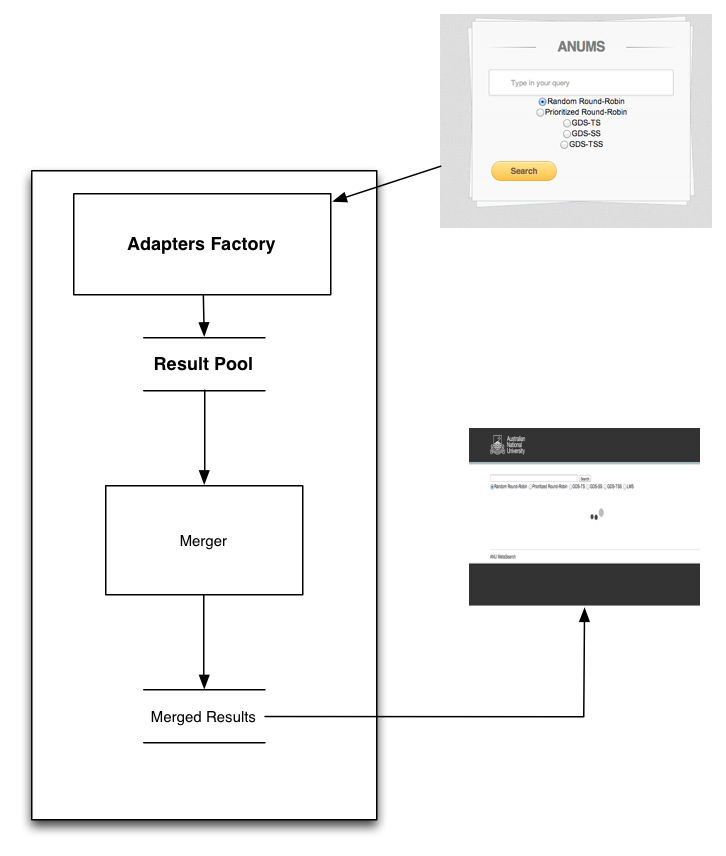
\includegraphics[width=0.6\textwidth]{MS_ARC.jpg}
\caption{The architecture of meta-search}
\label{fig:ms_arc}
\end{figure}
The main components of the broker are \textit{search interface adapter} which analyse each result page of individual search engine, and \textit{merger}  which fuses the results in a particular algorithm and returns the result. Figure \ref{fig:ms_arc} is an architecture of the meta-search system. We provide a search engine user interface to input the queries. The web will submit the query to the broker when a query search action is taken. The broker read the query and pass the it to the adapter factory. The adapter reads each query and pass it to its parser, the parser analysis the result page of each component search engine and put the result into a result pool. The merger will read result lists from the result pool and execute merging using a particular algorithm and then return the merged list.

The other parts is \textit{Evaluation System}, which is used to evaluate the performance of different algorithms and provide statistical as well graphic form of performance. The essential function of the evaluation system is as follows:
\begin{itemize}
\item Initial a test collection using the meta-search engine.
\item Provide a relevance judgement interface to assessors and record the graded relevance score on a query and documents.
\item Executing result merging of different algorithms and record the fused list of each query.
\item Compare the results with user judgements.
\end{itemize}
The evaluation system use the facilities of the meta-search to initialize the test collection, namely the document pages as well as statistical information of the results. The system also provide a relevance judgement system to assessor the judge the relevance scores between queries and documents. A component named algorithm evaluator is the core function of the system, which execute different merging algorithms on the broker and store the result lists. The algorithm evaluator will output varies performance information based on different criteria.

\begin{figure}
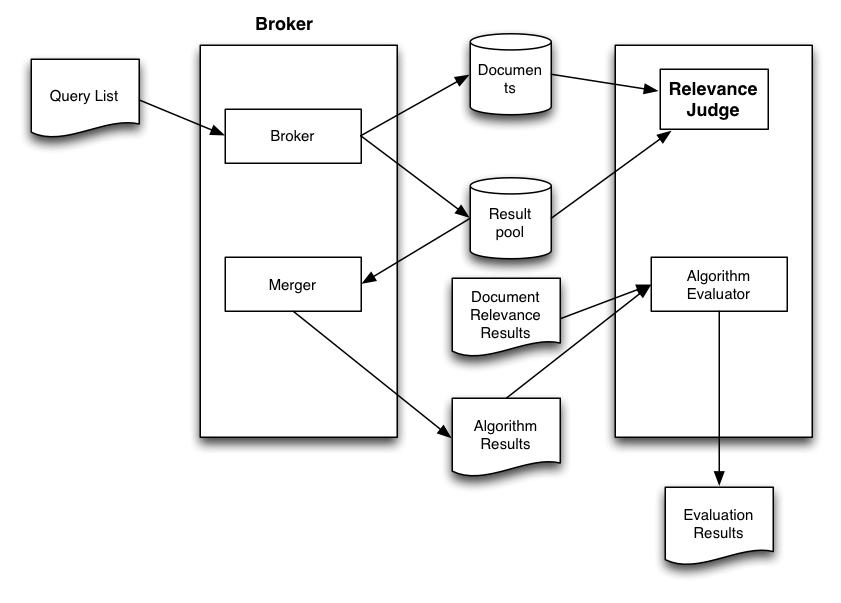
\includegraphics[width=1\textwidth]{eva_arc.jpg}
\caption{The architecture of evaluation system}
\label{fig:eva_arc}
\end{figure}  


\section{Methodologies}
We examined many of the algorithms discussed in the literature review and fit in some of the algorithms that is suitable for this environment.
\subsection{Round-Robin}
Round-Robin was used as a common method in many of the previous works in meta-search. The advantage   of round-robin is that it preserve the original rank of documents in a collection. However, the relative order of a document of a collection to a document in another collection is quite random. For example, in our environment, we have more than 10 document collections in total. If we have a collection that contains many comprehensive relevant documents but ranked at end of each round-robin cycle, the most relevant document will rank low in such a case. The other disadvantage of round-robin is that it holds a hypothesis that documents are distributed evenly in each collection, which is not accurate in a real world situation. We implemented a round-robin method in the experiments and use it as the baseline of all the algorithms. The order of documents in each cycle is determined by collections that is randomly ordered.
\subsection{Prioritized Round-Robin}
One drawback of round-robin method is as we talked above that they rank documents randomly in each cycle. To reduce the random effect of round-robin, we try to rank collections in advance according to the relevance of the collection and the query. Collections is biased on a query because a particular collection may focus on some particular topics. There are many algorithms in previous study doing collection selection calculate the collection weight according to some provided statistical information of the collection. However, in our environment, there is limited information on the collection. The only statistical information on collection when doing a search are the length of documents that retrieved by that collection as well as the result page.The length of documents that retrieved by different collections is potentially an indication of collection significance. We used the LMS method to get a collection score and rank collection by the collection score. We have already stored the length of retrieved documents when initializing the test collection. The algorithm first calculate the LMS scoring using the document length before doing the round-robin.

The result page reveals some information on the collection. We develop an algorithm using the average document similarity as a collection score. For documents ${d_1, d_2, d_3,...,d_n}$ in collection ${C_i}$, the average similarity $W_i$ is calculated as follows:
\begin{equation}
\label{eq:average similarity}
W_i=\frac{\sum\limits_1^N s_i}{N}
\end{equation}
, where $s_i$ denotes the similarity of $d_i$ and the query.

The same as the LMS based prioritized Round-robin, the merger get each collection's score at first and then rank the collections in the order of collection score. The merged list will be outputted in a round-robin mechanical following the collection order.

\subsection{Generic document scoring}
The score estimation methods proposed by \cite{Rasolofo2003} is a more practical approach in such a situation that there exist limited information on the original score assigned by each collection as well as collection statistics. The method used different textual fields that is available to public users as a representation of document topics. This fields are easy and cheap to obtain. And in most of case, these filed are summaries of what the documents talking about, which is a good indication of document focus. The score of a document is calculated by the generic document scoring function of Equation \eqref{eq:dscore} using the frequency of query terms that appears in the filed. In this experiment, we used four methods derived from the scoring functions. The first one that we used is the title field, the method is named \textit{SM-TS}, namely the document title scoring. As it is stated by \cite{Rasolofo2003}, the document title returned by the search engine is more accurate and reliable. And most of search engines return a document summary to display some key contents of the retrieved documents. So we also used \textit{SM-SS}, namely document summary scoring, by getting the document score using the generic function score. Furthermore, We utilized the combining method using both document title and document summary. The title is sometime too short and query terms may not be contained in the title. Also, in many cases, the query terms and some terms in the field may have the similar semantic information but expressed by different words. So the score for many relevant documents may remains to be zero in such a case. So we use the score of summary field as a supplement when the title score is zero. Algorithm \ref{al:TTS} illustrates the scoring function we used in the TSS method. Notice that rank score is applied when the two other scoring function failed. To keep the significance of filed core, we divide the rank score by 10,000 to make sure that documents that has a filed score will not be ranked higher than those document without a zero score. The rank score is simply calculated by $RS=(10-R+1)/10$, in which RS denotes the rank score and R denotes the rank of the document in the collection.  

\begin{algorithm}
\caption{TSS Scoring algorithm}
\label{al:TTS}
\begin{algorithmic}
\State{$TTS=TS$}
\If{$TTS==0$} 
	\State{$TTS=SS$}
	\If{$TTS==0$}
		\State{$TTS=RS$}
	\EndIf
\EndIf
\end{algorithmic}
\end{algorithm}



Also \cite{Rasolofo2003} suggested that the combining method can be implemented by giving different weights to title score and summary score as Equation \eqref{eq:DTSS}. The weight $k$ and $1-k$ are given to title score and summary score respectively and both in the range from 0 to 1. We also add a rank score to get rid of zero score. The constant $k$ shows the importance of title score and summary score. We'll test the value in our experiments later on.

\begin{equation}
\label{eq:DTSS}
DTSS=k*TS+(1-k)*SS
\end{equation}

\subsection{Length-based collection score}
As discussed above, the number of documents retrieved by each collection may be a good indication of collection relevance. We tried to use the method \cite{Rasolofo2001} proposed, and calculate the collection weight by Equation \eqref{eq:lms} and Equation \eqref{eq:lms_weight}. The method is just a way to give the collection weight. It has been used in the round-robin method as a collection score. In this method, however, we combine the weight by the estimated score obtained by the DTSS method to show if the performance has been improved. So we now get a score $S_{ij}$ for a document $d_i$ in collection $C_j$ by Equation 
\begin{equation}
\label{eq:lms_dtts}
S_{ij}=w_j*DTTS_i
\end{equation}
, in which $w_j$ denotes the collection weight of collection $C_i$.

\subsection{Locally re-index}
A more reliable way to conduct the result merger is to build another index system locally and conduct retrieve based on the index system. So when a search action is taken, the system download the documents documents retrieved by all the component search engines and build an index file based on the documents. The system then will calculate the document score based on the scoring function and return the documents in a list ordered by document score. In our experiments, all the documents retrieved by all the search engines have been downloaded to the local disk as we build the test collection, so in our locally re-index algorithm, when doing a search on a particular query, the merger retrieves the results from locally stored result pool and reads corresponding documents from test collection into memory. We used the open source Java library Lucene to index and score the documents. As the Lucene library returns just the relevant documents judged by itself, we put other documents at the end of the list.

Locally re-index is said to be accurate and reliable in its nature. However, the process of downloading and indexing is quite time consuming. It might not be a practical approach in a real world situation due to large volumes of documents and the limitation of bandwidth as well as users' patience. However, we implemented the algorithm in our experiment as a benchmark. So if an algorithm can outperform, or  be as good as the locally re-index algorithm, it is quite acceptable.
   

\subsection{Multiple Weight}

As we can see from what we have discussed above, the actual rank of documents is influenced by many factories. But however, it is not clearly for us at the moment that how these factors effect the final ranking. So in this experiment, we try to build a model that take all these factors into consideration and find out the weights for each of these factors.
The information can be achieved from a typical uncooperative federal search environment is as follows:
\begin{itemize}
\item
The similarity between the document title of a document $d_i$ and the query, denoted by $TS$.
\item
The similarity between the document summary of a document $d_i$ and the query, denoted by $SS_i$.
\item
The number of documents that are retrieved by a collection $C_i$, denoted by $N_i$
\item
The average similarity of the documents in a collection $C_i$, denoted by $aveS_i$
\item
The rank score given by the collection for a query $R_i$
\end{itemize}
The first two information belongs text field that can be used to estimate the document similarity. A previous research has been done by \cite{Rasolofo2003} using a generic document function to estimate the document similarity, as we discussed. And the number of document retrieved as well as the average document similarity reveals the significance of a collection to a particular topic. The last factor, rank score, demonstrate the original ranking of a document in a collection. The original rank of a document in a collection is ignored by most of the score based algorithms, As a matter of fact, although rank score of a document does not show exactly the score of a document assigned by the component search engine, it shows the order of document scores. And whether we should preserve the original order of document ranking remains to be research question. Algorithms like round-robin can outperform other algorithms in some cases is because the original rankings of component search engines are quote good and even. So as round-robin preserve the goodness of the original ranking, it outputs a good ranking. We built a linear regression model utilizing these factors: 

\begin{equation}
\label{eq:mul_col}
S_i=w_1*LMS_i+w_2*aveS_i+w_3*Eds_i+w_4*Rs_i
\end{equation}
, where $S_i$ denotes the score for document $d_i$, and {$w_1$, $w_2$,$w_3$,$w_4$} denotes the weights assigned to these factors respectively. The document length score, denoted by $LMS_i$ is calculated using the length based scoring function proposed by \cite{Rasolofo2001}. $Eds_i$ denotes the estimated document similarity using generic document scoring function and $Rs_i$ is the rank score of document $d_i$ in its original collection.

The remain problem became how to estimate theses weights. In SSL method\cite{Si2003a}, they proposed a similar approach by building such a regression model to map original document score to a document score in the sampling collection. However, in our experiment, the sampling data is not practical to achieve. Instead, we build a linear regression model which map these four factors to the relevance score. So the intended linear function becomes:
\begin{equation}
\label{eq:regression}
f(w,x_i)=w_1*LMS_i+w_2*aveS_i+w_3*Eds_i+w_4*Rs_i
\end{equation}
And to solve this problem, we used a least square method in linear regression. The aim of the model is to find a set of parameters, which minimise the square difference between the function and the relevance score.
\begin{equation}
\label{eq:leastsquare}
w=arg \min\limits_w{\sum\limits_{i}(f(w,x_i)-rel_i)^2}
\end{equation}
The ideal relevance score is already be assessed by assessors, we'll use a n-fold cross validation method to test the performance of this function. We separate the 44 queries that we experimented into 4 folds, each contains 11 queries. And We pick three of the fold as the training data and keep the remain as the testing data. The testing is comprised of those factors as well as the relevance score assessed.


\subsection{Unimplemented Algorithms}

Not all of the algorithms that we discussed in literature review were implemented due to the limitation of information available. First of all, as we discussed in literature review, some algorithms can only be used in Aggregated meta-search. A fundamental condition of implementing this kind of algorithm is that there is sufficient amount of document overlap among different collections. However, there exist just little or no document overlap in most of the result returned by different collections in our experiments environment. The environment that we use in this experiment is a typical model of non-aggregated meta-search. So those aggregated merging algorithms were not considered in the experiments.
  
CORI is well-known distributed information retrieval resolution in collection selection. A merging algorithm is also come along with it. The merging algorithm of CORI calculates collection weights by normalizing the collection scores that are obtained in the collection selection step. The original CORI system is built upon the INQUERY system, which constructs an inference network based on probability. And the building of the INQUERY system requires collaboration of the collections. Even if we do not use INQUERY system to get collection score using CORI algorithm, some statistical information on the collections are needed. 

For a term $t_k$, we calculate the belief that term $t_k$ can be observed by the collection, namely $p(t_k|c_i)$ by:

\begin{equation}
T=\frac{df}{df+50+150\cdot cw/avg\_cw}
\end{equation}

\begin{equation}
I=\frac{\log(\frac{C+0.5}{cf})}{\log{(C+1.0)}}
\end{equation}

\begin{equation}
p(t_k|c_i) = b+ (1-b)\cdot T\cdot I
\end{equation}
$df$ is the number of documents in a collection $C_i$ contains a term, $cw$ is the number of terms in $C_i$, $avg_cw$ is the average $cw$ of all the collections. $C$ is the number of collections, $cf$ is the number of collections that contain the term. $b$ is a constant, usually set to 0.4. So to get a collection score for a query, we need to get the $p$ for each term appears in the query and aggregate them in some methods. And then we use a minmax method to normalize the collection scores to get a collection weight, the collection weight is then combined to other raw score functions. So, as far as we can see, the utilization of CORI algorithm requires basic term size and document frequency of a collection, which is not available in our case.

As we discussed above, machine learning approaches can be promising methods in solving meta-search merging problems. For example, the SSL method using regression method to map the document score in the original collection into an integrated index centralised sampling collection. Issues arise when sampling the document collections. First of all, the size of each collection is unknown, so it becomes a tricky problem how many documents should we keep to form the collection sample. And on the hand other, the documents in each collection are not static due to the characteristic of web collection, it is hard to guarantee the accuracy of the sample. The sample size should large enough so that there exists at least three document overlap in each query result, in which case, the sampling process would be very time  and capacity consuming.

There exists other machine learning methods which build clustering or document distribution based on previous queries. So to execute these methods, we need training data to construct the model. Due to the limitation of usage of the platform, it is hard to achieve enough training data. As a matter of fact, users tend to use short and inaccurate query terms to express their information needs, which means that the correlation between queries is very small. So if we put them into a machine learning model, the similarities between new queries and past queries are too tiny. 

\section{Evaluation Criteria}
We chose  several criteria to demonstrate the performance of the algorithms, both binary and non-binary. Although as we discussed about, binary relevance is not sufficient to prove the efficient of an algorithm, it is still a common criteria that would be used in the evaluation of information retrieval system. Because all the algorithms run on the fixed result pool that is initialized in advance. So the recall as well as precision are the same for all the algorithms. However, different algorithm rank documents in different order, so the precision as well as recall of different algorithms at position k varies. So the basic criteria that we use to measure the performance is \textit{Precision at k}.

\begin{equation}
\label{eq:prec10}
Prec@10=\frac{|Top\ 10\ retrived\ Documents\cap Relevant\ Documents|}{10}
\end{equation}

As we preserved the top 10 documents from each collection. It seems like that many of document would be relevant to the query because they are already ranked high by their ranking system. However, for two different documents that are relevant to a topic, the degree of relevance varies. Some documents may mention part of the topic while others may exactly focus on the topic. So if the a system can rank more relevant document higher than less relevant documents, it is better than others. Due to the unbalanced relevance score of different documents, we applied a graded judgement method, NDCG, which use cumulated score with respect to the ideal ranking. We generate the NDCG result for each algorithm of a query and graphic representation of the NDCG.

\section{Relevance judgement}

The document judgement procedure gives a score to the relevance of documents and the query. The relevance score then will be used in the evaluation of merging algorithms as a benchmark or ideal ranking. Conventional test collections invite experts from a specific domain to assess the relevance score, and typically, the relevance of documents with respect to a query is judged as binary score, namely \textit{relevant} and \textit{irrelevant}. However, as we discussed before, binary relevance method is not sufficient to prove that an information retrieval system is better than other. So, in this experiment, we used non-binary relevance judgement method. The relevance of documents and queries were assigned to 5 levels, namely \textit{irrelevant}, \textit{On-topic but useless},\textit{Somewhat useful},\textit{Useful},\textit{Comprehensively useful} and the criteria of relevance is given as follows:

\textbf{\emph{Irrelevant}} is the score given to documents that are totally irrelevant to the topic.

\textbf{\emph{On-topic but useless}} is the score given to documents that are related to the topic but is talking on some other aspects of the area.	

\textbf{\emph{Somewhat useful}} is the score given to documents that are relevant to the topic and the topics that the queries are intended to retrieved are mentioned in the documents.

\textbf{\emph{Useful}} is the score given to documents that most, or at least some part of the documents are talking on the intended information.

\textbf{\emph{Comprehensively useful}} is the score given to the documents that are talking exactly on the topic.

According to these 5 level of relevance, we set the relevance score in the range from 0, which is irrelevant, to 4, which is given to documents that is comprehensive.

\begin{figure}	
\centering
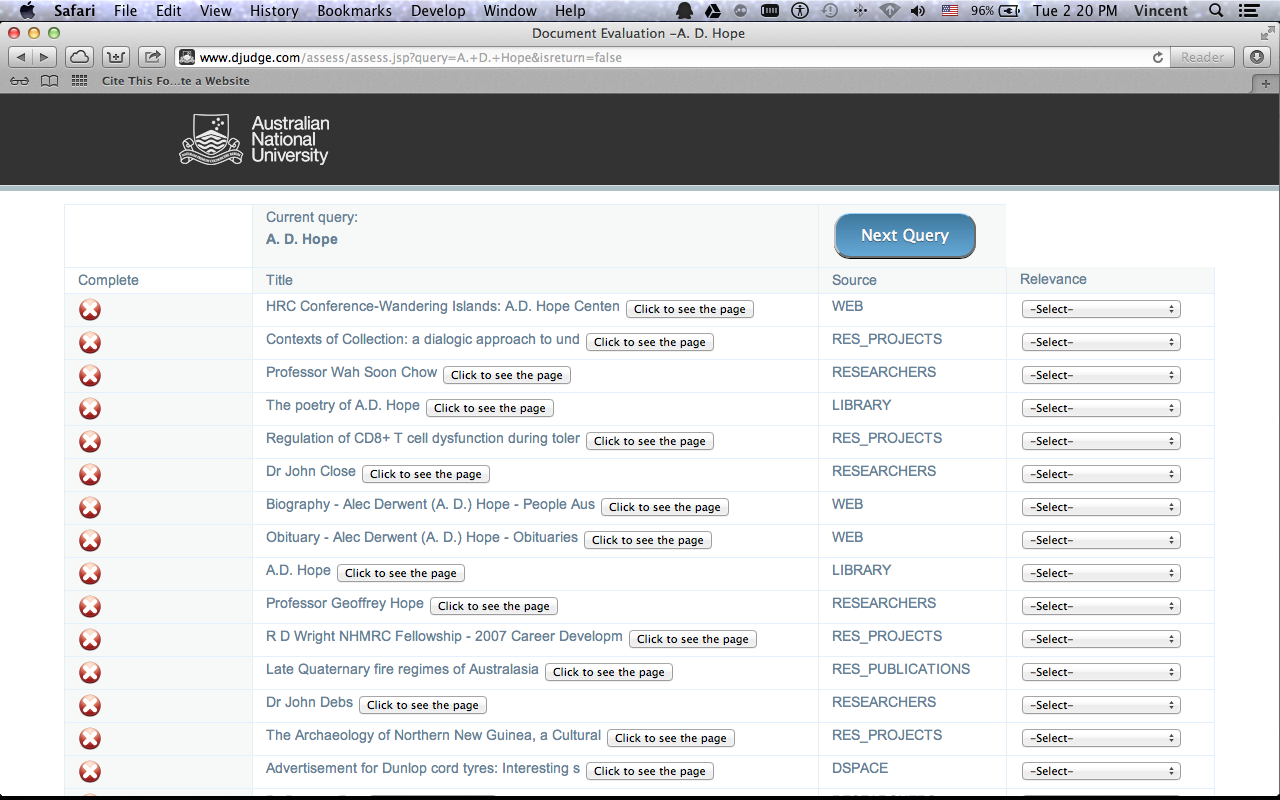
\includegraphics[width=0.8\textwidth]{djudge.png}
\caption{User Interface of Document judgement system}
\label{fig:djudge}
\end{figure}
We set up a web-based platform for assessors to conduct the assessing process. The platform provides a solid user interface, in which a particular query and its potential relevant documents are provided. Assessor can pick up a query can assess each document using the platform. 

\section{Experimental Procedure}
We separated our experiment into several stages, the first of which is initializing the test collection and experiment platform. In this stage, we initialized the test collection by passing the query list to the broker. The broker retrieved the result documents from each collection and store the original documents as well as the result pool locally. The next step is conducting relevance judgement. We set up a web-based judgement system on-line. We also set-up a relational database (Mysql) bounding to the website to store the query and its corresponding documents. We invited 20 volunteers of different background from the Australian National University, who are also potential users of the system. Although people from different backgrounds may have biased on information needs and may generate different relevance results, we do not record personal information in our experiment for several reasons. First of all, to secure the individual privacy, it is more safe to get rid of these personal information and is a policy of the university to protect personal information in a research project. And on the other hand, the research is focused on the merging algorithm regardless of the influence of personal feedback. And also, the topics that we pick up are very common and are not ambiguous to any person in any background, which is intend to eliminate the personal effect. 

We set up a web-based document judgement system on-line, the system is developed using JSP technique and is deployed in an Apache Tomcat sever on a Linux system. The system provide a user interface as the platform of the experiment. To keep the completeness of the document score, we added a feature for user that they can continue assessing the query after a period of time. Assessors were trained to use the application as well as how to score the relevance properly before the execution of the experiments. 

After all the queries have been assessed, we gather the document judgement result to local xml file. The final stage is to evaluate the performance of different algorithm according to the relevance score. In this stage, we run different algorithms on the query list and output the ranking results of these algorithms. Again, we store the result of these algorithms in xml file query by query. We pass the algorithm result as well as our user judgement document to an evaluation script that we wrote based on different criteria and get results of their performance.


